\section{Experiments}
\label{sec:results}
To demonstrate our superiority over existing methods on segmentation, we first present results on two diverse biomedical image segmentation problems, including synaptic vesicle segmentation and gland segmentation.
To demonstrate the easy extension and generic applicability of our framework, we modified our SCNN to scene text segmentation task.

\subsection{Synaptic vesicle segmentation}
\noindent\textbf{Dataset}
Synaptic vesicle is a good example to evaluate our method, as most of vesicle shape are ellipse.
The images were acquired by . \cxj{by what?}
However synaptic vesicle images are much noisy due to.
The plausible vesicles in image are densely arranged and easily confused with other membrane in presynaptic cell, therefore it is hard to obtain clear contour for such dense and small objects.
%The ground truths of dataset are held out by biologists for objective evaluation.
The original dataset is composed of $120$ images with annotations provided by biologists.
The height and width of each image are respectively $1019$ and $1053$, averagely containing $200$ vesicle objects.
Since the average length of a vesicle is about $30$ pixel, we crop a $321\times 321$ region from the original image as our input to network so that each cropped image contain about $25$ objects.
We uniformly crop $25$ patches in each original image with overlap, then the final dataset consists of $3000$ images of $321\times 321$ resolution.
\cxj{image size?}

Similar with many existing approaches, we utilize a data augmentation process to reduce the overfitting and increase the robustness of our network.
In the data augmentation, translation, rotation and image flipping are used, which generate total $8787$ images.
\cxj{The final dataset size?}

For better evaluation, a six-fold cross validation is applied in our experiments.
The first five out of six images are prepared to train our model and the rest of them are used to test its performance.
\cxj{Six-fold cross validation? or other strategy? }
%
The validation processing has been repeated several times and the average performance will be reports.


\noindent\textbf{Implementation details.}
We train our network on the open-source deep learning library Caffe~\cite{Jia2014}.
%All the experiments are implemented on a workstation with TitanX GPU cards.
The model of our SCNN is well trained by two-step process.
In first stage, we independently train the segmentation branch and shared layers as a general segmentation task.
The parameters of shared layers are initialized from VGG-16 ImageNet pretrained model.
During training phase, the base learning rate was set as $10^{-3}$ and a 'step' policy is adopted by decreasing the learning rate by a fact of $10$ every $2000$ iterations.
And mini-batch size was set to $30$ for one iteration with the max iteration number $20k$.
In the second stage, the multi-task FCN as well as two successive joint max pooling layers is jointly fine-tuned on the model from first stage.
The learning rate of new added layers in auxiliary branch was set as $10^{-5}$, while the other learning rate was set to $10^{-8}$.
The iteration number of second stage isset as $8k$.
For max pooling layers, pooling size was set as $7\times 7$ with stride $1$.
And the balancing weight $\lambda$ in Eq.~\ref{EqLoss} was set as $5$.
Finally because the shape of most vesicle contours are regular ellipse, we can impose a relative strong constraint to the shape of segmented objects.
Therefore in testing phase, the thresholds $\tau_1$ and $\tau_2$ in local fusion step are respectively set to $0.2$ and $0.9$.

\noindent\textbf{Evaluation setup.}
%
The evaluation criteria in our experiments includes an score $F_1$ to evaluate performance of object detection and a pixel intersection-overunion (IOU) averaged across different classes to evaluate the segmentation accuracy .
%The $F_1$ score considers the performance of object detection, while IOU consider the segmentation performance, respectively.

For detection, the $F_1$ score is defined as:
\cxj{Can we use a more intuitive symbol, say $R_{detection}$?}
%
\begin{eqnarray}\label{fusion}
\begin{aligned}
F1 = \frac{2PR}{P+R}
\end{aligned}
\end{eqnarray}
where $P$ is the detection precision and $R$ is the detection recall.
Especially, a true positive detection is the segmented object that intersects with at least $50\%$ with the ground truth, otherwise it is regarded as a false positive.
If a ground truth object has no corresponding segmented object that intersects more than $50\%$, it is regarded as a false negative.

The IOU metric for segmentation accuracy is defined as:
%
\begin{eqnarray}\label{fusion}
\begin{aligned}
IOU = \frac{1}{N_s}\sum_{i=1}^{N_s}\frac{G_i\bigcap S_i}{G_i\bigcup S_i}
\end{aligned}
\end{eqnarray}
%
where $N_s$ denotes the number of label classes.
$G_i$ denotes the pixel set in ground truth of $i$-th label.
$S_i$ denotes the pixel set in segmented map of $i$-th class.
In our object segmentation task, there are two kind of labels: object or background, therefore $N_s$ is set to $2$.
\cxj{What do you mean by "classes" here? instances? }

\begin{figure*}
    \begin{center}
        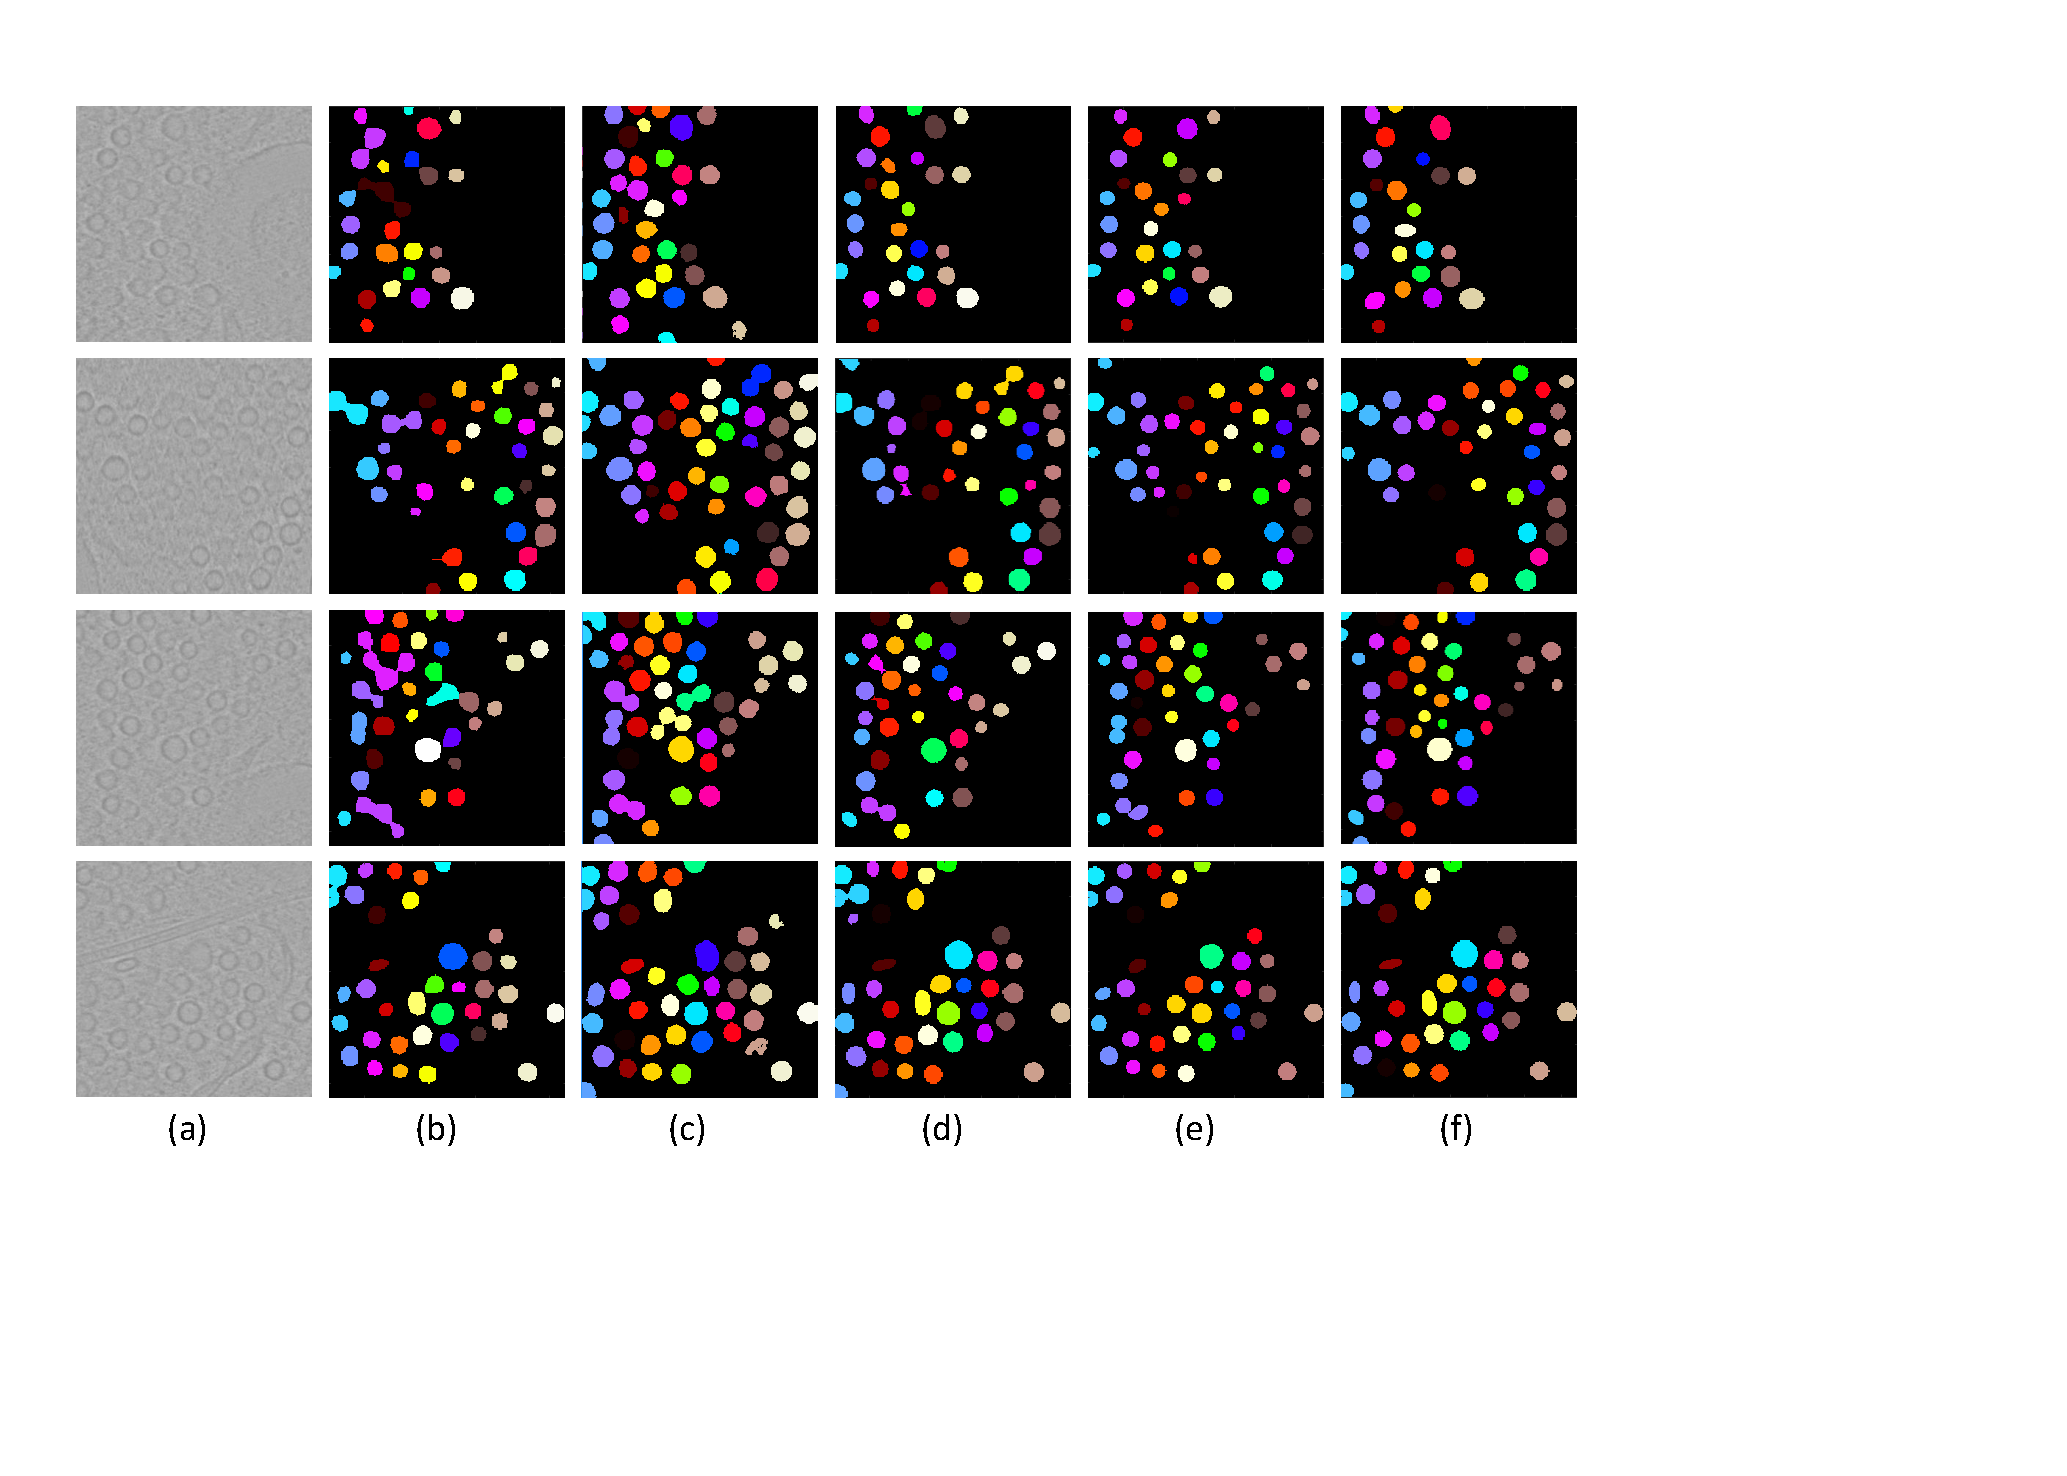
\includegraphics[width=6.8in]{figures/FigVesicle.pdf}
    \end{center}
    \caption{Some segmentation results of synaptic vesicle: the image from top to bottom are respectively input image, segmentation of u-net, DCAN, SCNN and ground truth.}
    \label{FigVesicle}
\end{figure*}


\noindent\textbf{Qualitative evaluation on synaptic vesicle segmentation}
Figure \ref{FigVesicle} shows some segmentation results of testing data.
In order to verify the effectiveness of parameterized shape information, we compared our method with DeepLab \cite{Chen2014a} without any complementary information and DCAN~\cite{Chen2016a} that uses auxiliary contour map.

From segmentation results we can see that without other complementary information, there exists many touching objects that cannot be separated by DeepLab (second row in \ref{FigVesicle}).
This is because that the contours of many synaptic vesicles are very fuzzy and even not complete that miss a part of membrane due to deficient imaging technology shown in first row in \ref{FigVesicle}.
Furthermore, as synaptic vesicles usually gather around presynaptic membrane, they are crowded together which increase the difficulty to separate them into individual ones.
Although DCAN is capable to separate touching synaptic vesicles apart in the third row of Figure \ref{FigVesicle}, it produced additional false positive detections between two touching vesicles.
The reason is that connection part between two touching vesicles are wide and long caused by terrible image quality, which can not be cleaned out by predicted contours.
Therefore in \cite{Chen2016a}, that the touching glands are closed is also a factor of success of DCAN, and we will present our SCNN still works for segmenting closed touching objects in our second experiments.
Differen from above two methods, our SCNN uses the shape parameters of objects as complementary information to separate the touching object clearly without any sequela.
The information in shape parameters of an object are more abundant, including the prior shape knowledge of segmented objects and main dominion belonging to the object.
As the results shown in forth row of Figure~\ref{FigVesicle}, all the touching objects have been well separated and their shape are more smooth and regular.
This demonstrates the superiority of our SCNN in segmenting densely arranged objects with regular and small objects by incorporating the prior shape knowledge into network.

\noindent\textbf{Quantitative evaluation.}
To quantitatively evaluate our method, we compare the object detection rate $F_1$ and the segmentation accuracy IOU of our SCNN with the state of the art segmentation methods based on Deeplab~\cite{Chen2014a}, u-net~\cite{Ronneberger2015} and DCAN~\cite{Chen2016b}, which are commonly used in biomedical image process.
%
Their results on our synaptic vesicle dataset are shown in Table~\ref{tab:vesicle}.
%
And we further implement two version of SCNN.
The first SCNNv1 is the implementation of multi-task neural network without joint max pooling, and SCNNv2 is the complete form.
Their results are also presented in Table~\ref{tab:vesicle} to prove effectiveness of our joint max pooling.

From F1 score obtained in Table~\ref{tab:vesicle}, the performance of SCNN surpassed the other methods.
The common low F1 scores are caused by difficulty in detecting dense synaptical vesicles in such noise background.
Especially, we observed that the performance of u-net obtained about $3\%$ improvement over DeepLab, both of which didn't use any auxiliary supervised information.
This arises from the fact that U-shape applied in u-net is effective to alleviate touching problem by supplementing many context information to higher resolutions layers.
It confirmed that deficiency of context information due to successive pooling and downsampling layers is a significant factor of touching problem in biomedical segmentation.
Furthermore, we noticed that F1 score of DCAN turns out to be the worst among all the methods.
This mainly comes from the extra patch between two objects that are original touched and separated by predicted contours, shown in Figure~\ref{FigVesicle}.
Many these extra patches increase the false positive counts of DCAN.
And it can be seen that our joint max pooling operation significantly improve the performance of using shape parameter as auxiliary information.

From IOU metrics in Table~\ref{tab:vesicle}, our SCNN again gives the best performance among various methods.
It should be noted that although the other methods also obtain a good IOU score, their contour are more coarse and irregular, which increase the difficulty of post-processing such as reconstruction of 3D synaptic vesicle structure.
And our segmented vesicle are more clear and regular.


\begin{table}
\begin{center}
\begin{tabular}{lcc}
\hline
Method & F1 & IOU \\
\hline
DeepLab & 0.6675 & 0.8095 \\
U-net & 0.6999 & 0.7756 \\
DCAN & 0.7007 & 0.8533 \\
SCNNv1 & 0.7814 & 0.8857 \\
SCNNv2 & $\mathbf{0.8140}$ & $\mathbf{0.8984}$\\
\hline
\end{tabular}
\end{center}
\caption{The detection and segmentation results of different methods in our synaptic vesicle segmentation dataset.}
\label{tab:vesicle}
\end{table}





\subsection{Gland segmentation}
\textbf{Dataset}
In this section we present SCNN for segmenting benign and malignant gland.
We consider the public dataset of \emph{Gland Segmentation Challenge Contest} in MICCAI2015~\cite{Sirinukunwattana2015a}.
%
The training dataset is composed of 85 images, consisting of 37 benign and 48 malignant, with ground truth annotations provided by expert pathologists.
Especially, there is a huge variation of glandular morphology in malignant case, which can prove the generalization of our SCNN to irregular objects.
The same data augmentation in vesicle segmentation is implemented for a better performance.

\textbf{Implementation details}
Because there exists many irregular objects in gland images that we desire to remain more contour information obtained by object prediction, the contour modification by parameterized contour information should be relatively weaker than segmenting vesicles.
By experimental verification, we find that $\tau_2=0.7$ and $\tau_1=0.4 $ produce a better results.
\cxj{So show comparison of results using different parameters.}
%
And we still use the standard elliptic parameter as the prior shape constraint for gland, as most benign glands and few malignant glands' shape are approximate ellipses.
The other implementation settings and evaluation metrics follow the vesicle segmentation.

\textbf{Qualitative evaluation on gland segmentation}
Follow previous qualitative evaluation, we presented the results of u-net and the state of art method DCAN in gland segmentation with our SCNN in Figure~\ref{fig:com-gland}.
The first two columns are the examples of benign gland images, and the rest two columns are the examples of malignant images.
From the results, we can observed that both SCAN and SCNN can well solve the touching problem in benign and malignant cases.
However for benign case, the contours of glands obtained by SCNN are more smooth than that of DCAN.
And for malignant case, since SCNN only modify the segmentation predictions on the object border, there is no obvious deterioration compared to DCAN.

\begin{figure}
	\centering
	\vspace{0.4in}
	\caption{\cxj{Add comparison of gland segmentation with U-net and DCAN.}}
	\label{fig:com-gland}
\end{figure}

\textbf{Quantitative evaluation}
Table \ref{} shows the F1 score and IOU metric over the $Gland$ $Segmentation$ $Challenge$ $Contest$ by several commonly used biomedical segmentation methods.

\begin{table}
	\centering
	\caption{Performance comparison on gland segmentation.}
	\begin{tabular}{c|cc}
		\hline
		Method & F1 & IOU \\
		\hline
		DeepLab & 0 & 0 \\
		U-Net & 0 & 0 \\
		DCAN & 0 & 0 \\
		SCNN-v1 & 0 & 0 \\
		SCNN-v2 & 0 & 0 \\
		\hline
	\end{tabular}
\end{table}


\subsection{Scene text detection}
We further extended SCNN to scene text detection task, which
